\section{Geografska karta penjačkih lokacija}

Kako bi se korisnicima olakšala prostorna orijentacija, aplikacije integriraju interaktivnu geografsku kartu. Ova funkcionalnost omogućuje vizualno istraživanje penjačkih lokacija na globalnoj razini kao i detaljnu navigaciju unutar pojedinog penjališta.

\begin{figure}[H]
    \centering
    \begin{subfigure}[b]{\textwidth}
        \centering
        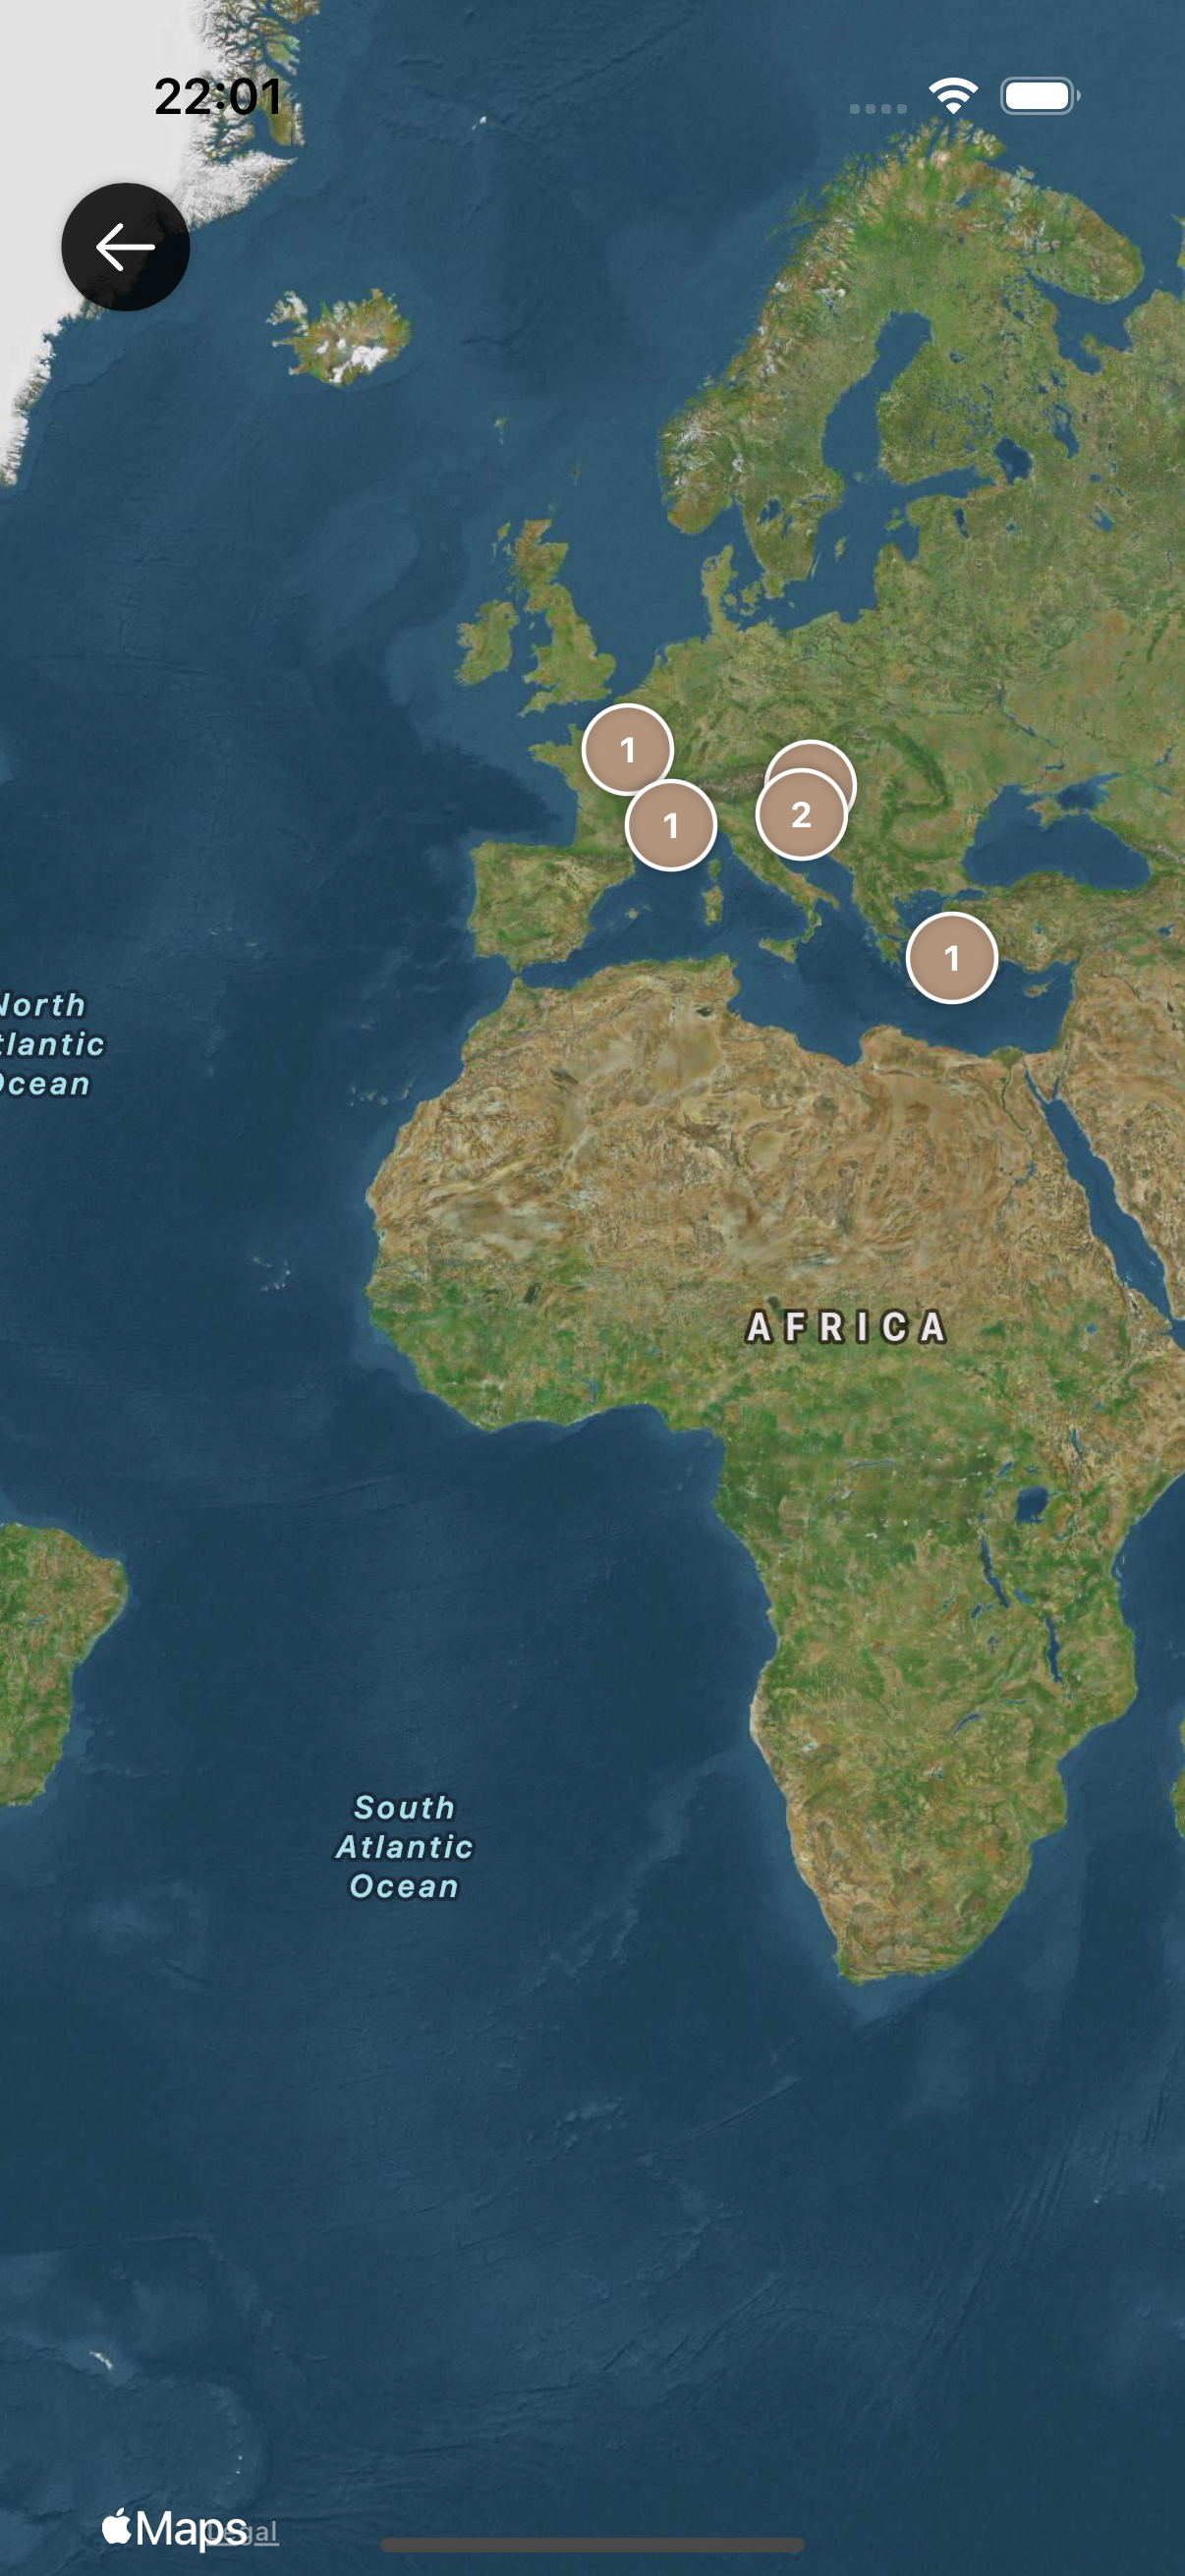
\includegraphics[width=0.3\textwidth]{images/implementacija/geo_karta.png}
        \caption{Mobilna aplikacija}
        \label{fig:geografska_karta_mob}
    \end{subfigure}
    \hfill
    \begin{subfigure}[b]{\textwidth}
        \centering
        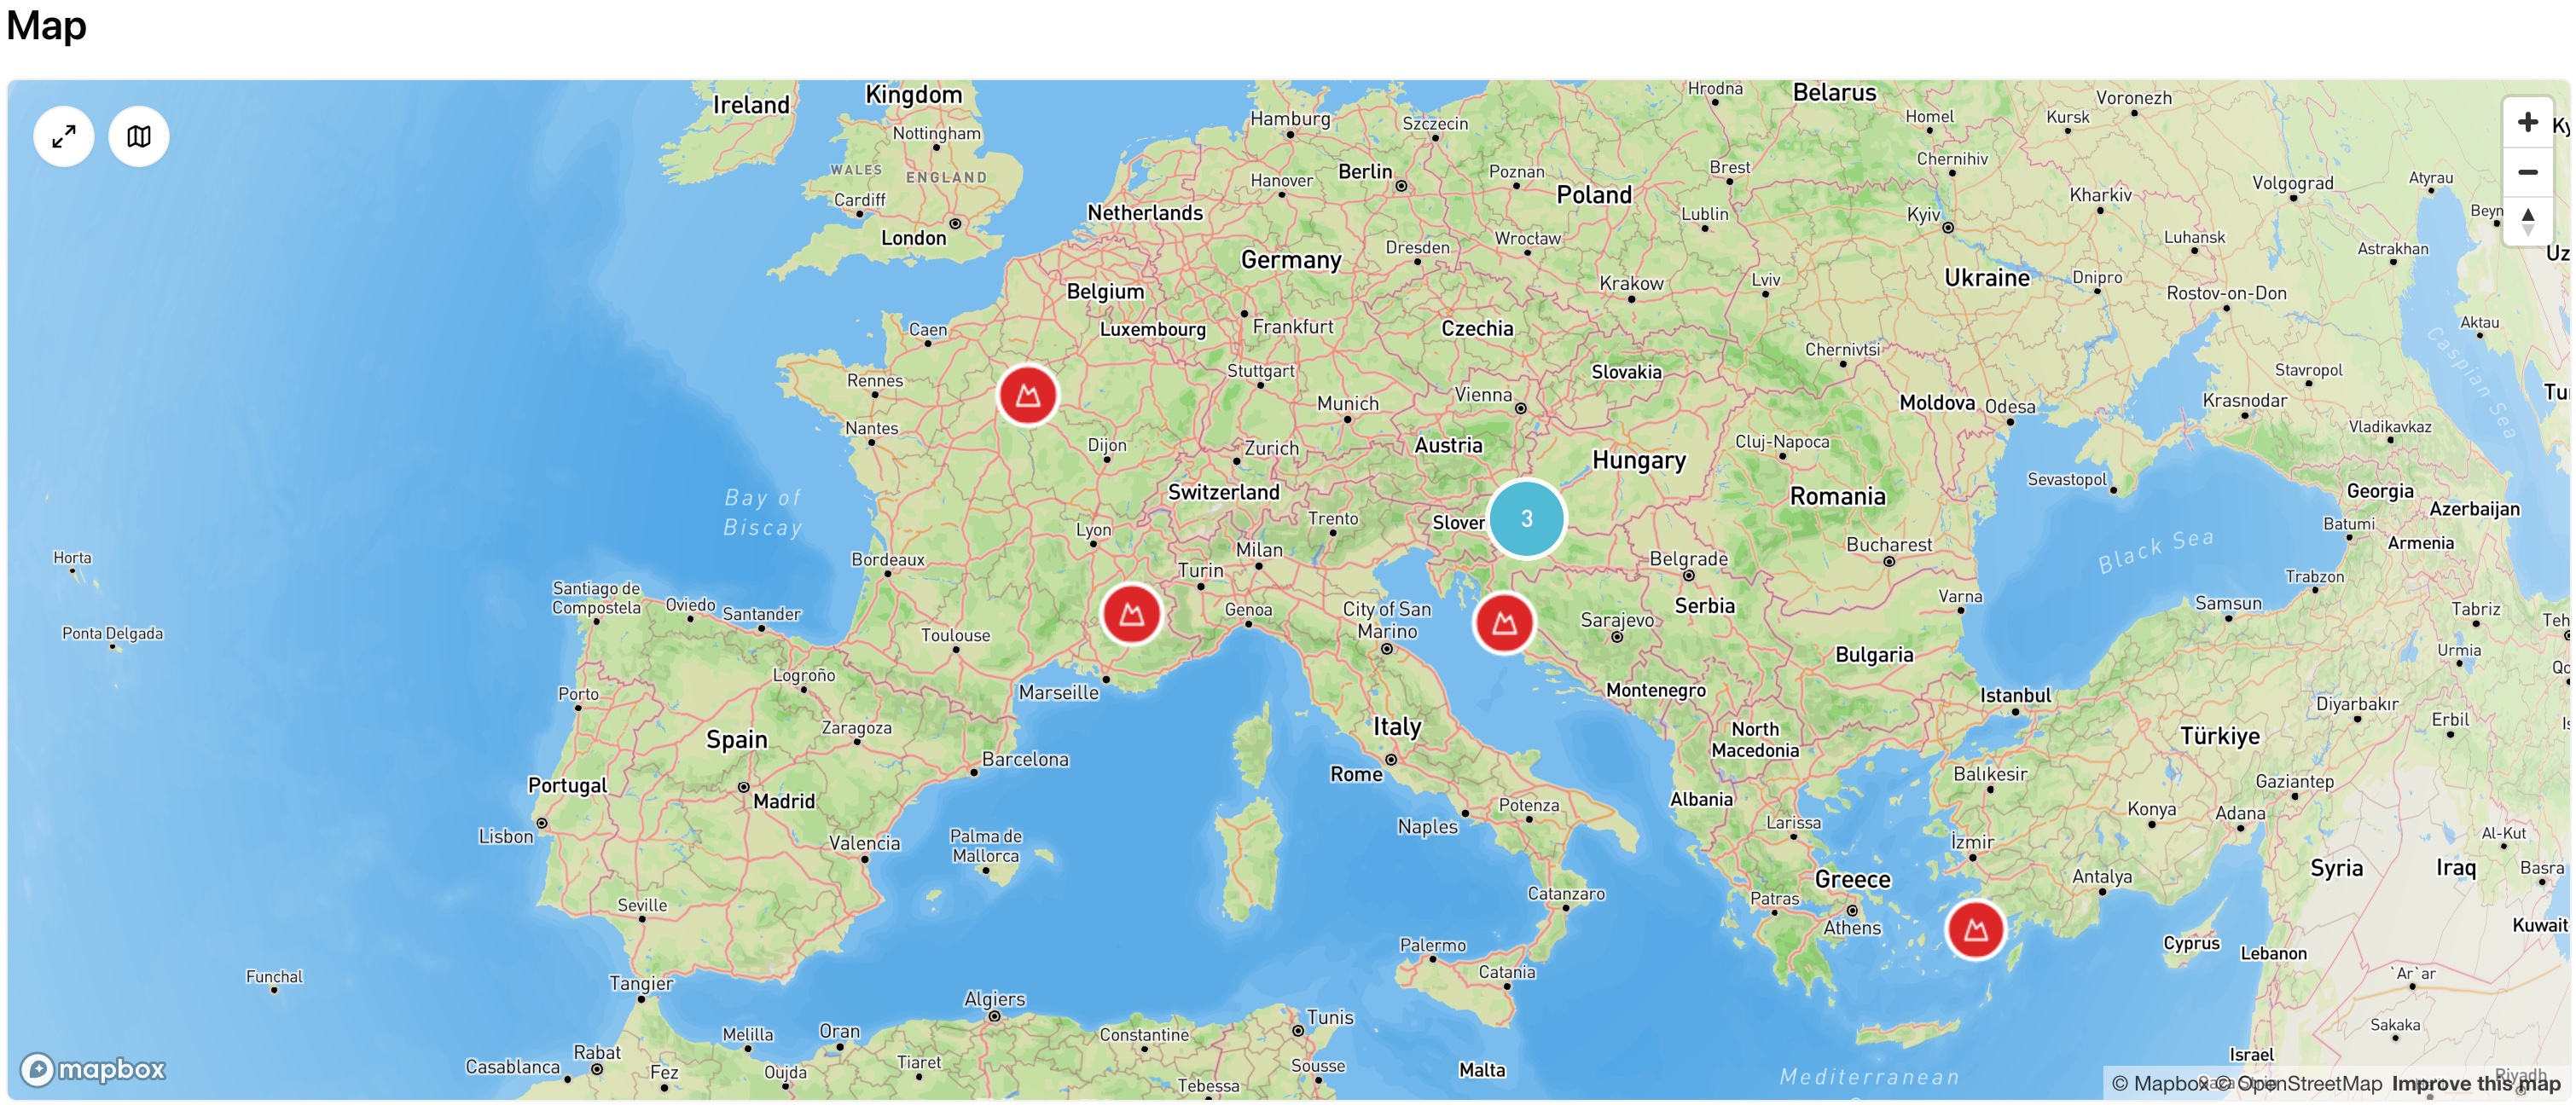
\includegraphics[width=0.9\textwidth]{images/implementacija/web/map_clusters.jpeg}
        \caption{Web aplikacija}
        \label{fig:geografska_karta_web}
    \end{subfigure}
    \caption{Geografska karta penjačkih lokacija s prikazom grupiranih oznaka}
    \label{fig:geografska_karta_sidebyside}
\end{figure}

Pristupom karti korisniku se prikazuje karta svijeta s grupiranim oznakama (eng. \textit{clusters}) koje indiciraju broj dostupnih penjališta na određenom području. Grupirane oznake omogućuju pregled prikaza na visokoj razini, ali bez pretrpanosti informacijama. Približavanjem karte, grupirane oznake se razdvajaju, otkrivajući pojedinačne lokacije penjališta.

\begin{figure}[H]
    \centering
    \begin{subfigure}[b]{\textwidth}
        \centering
        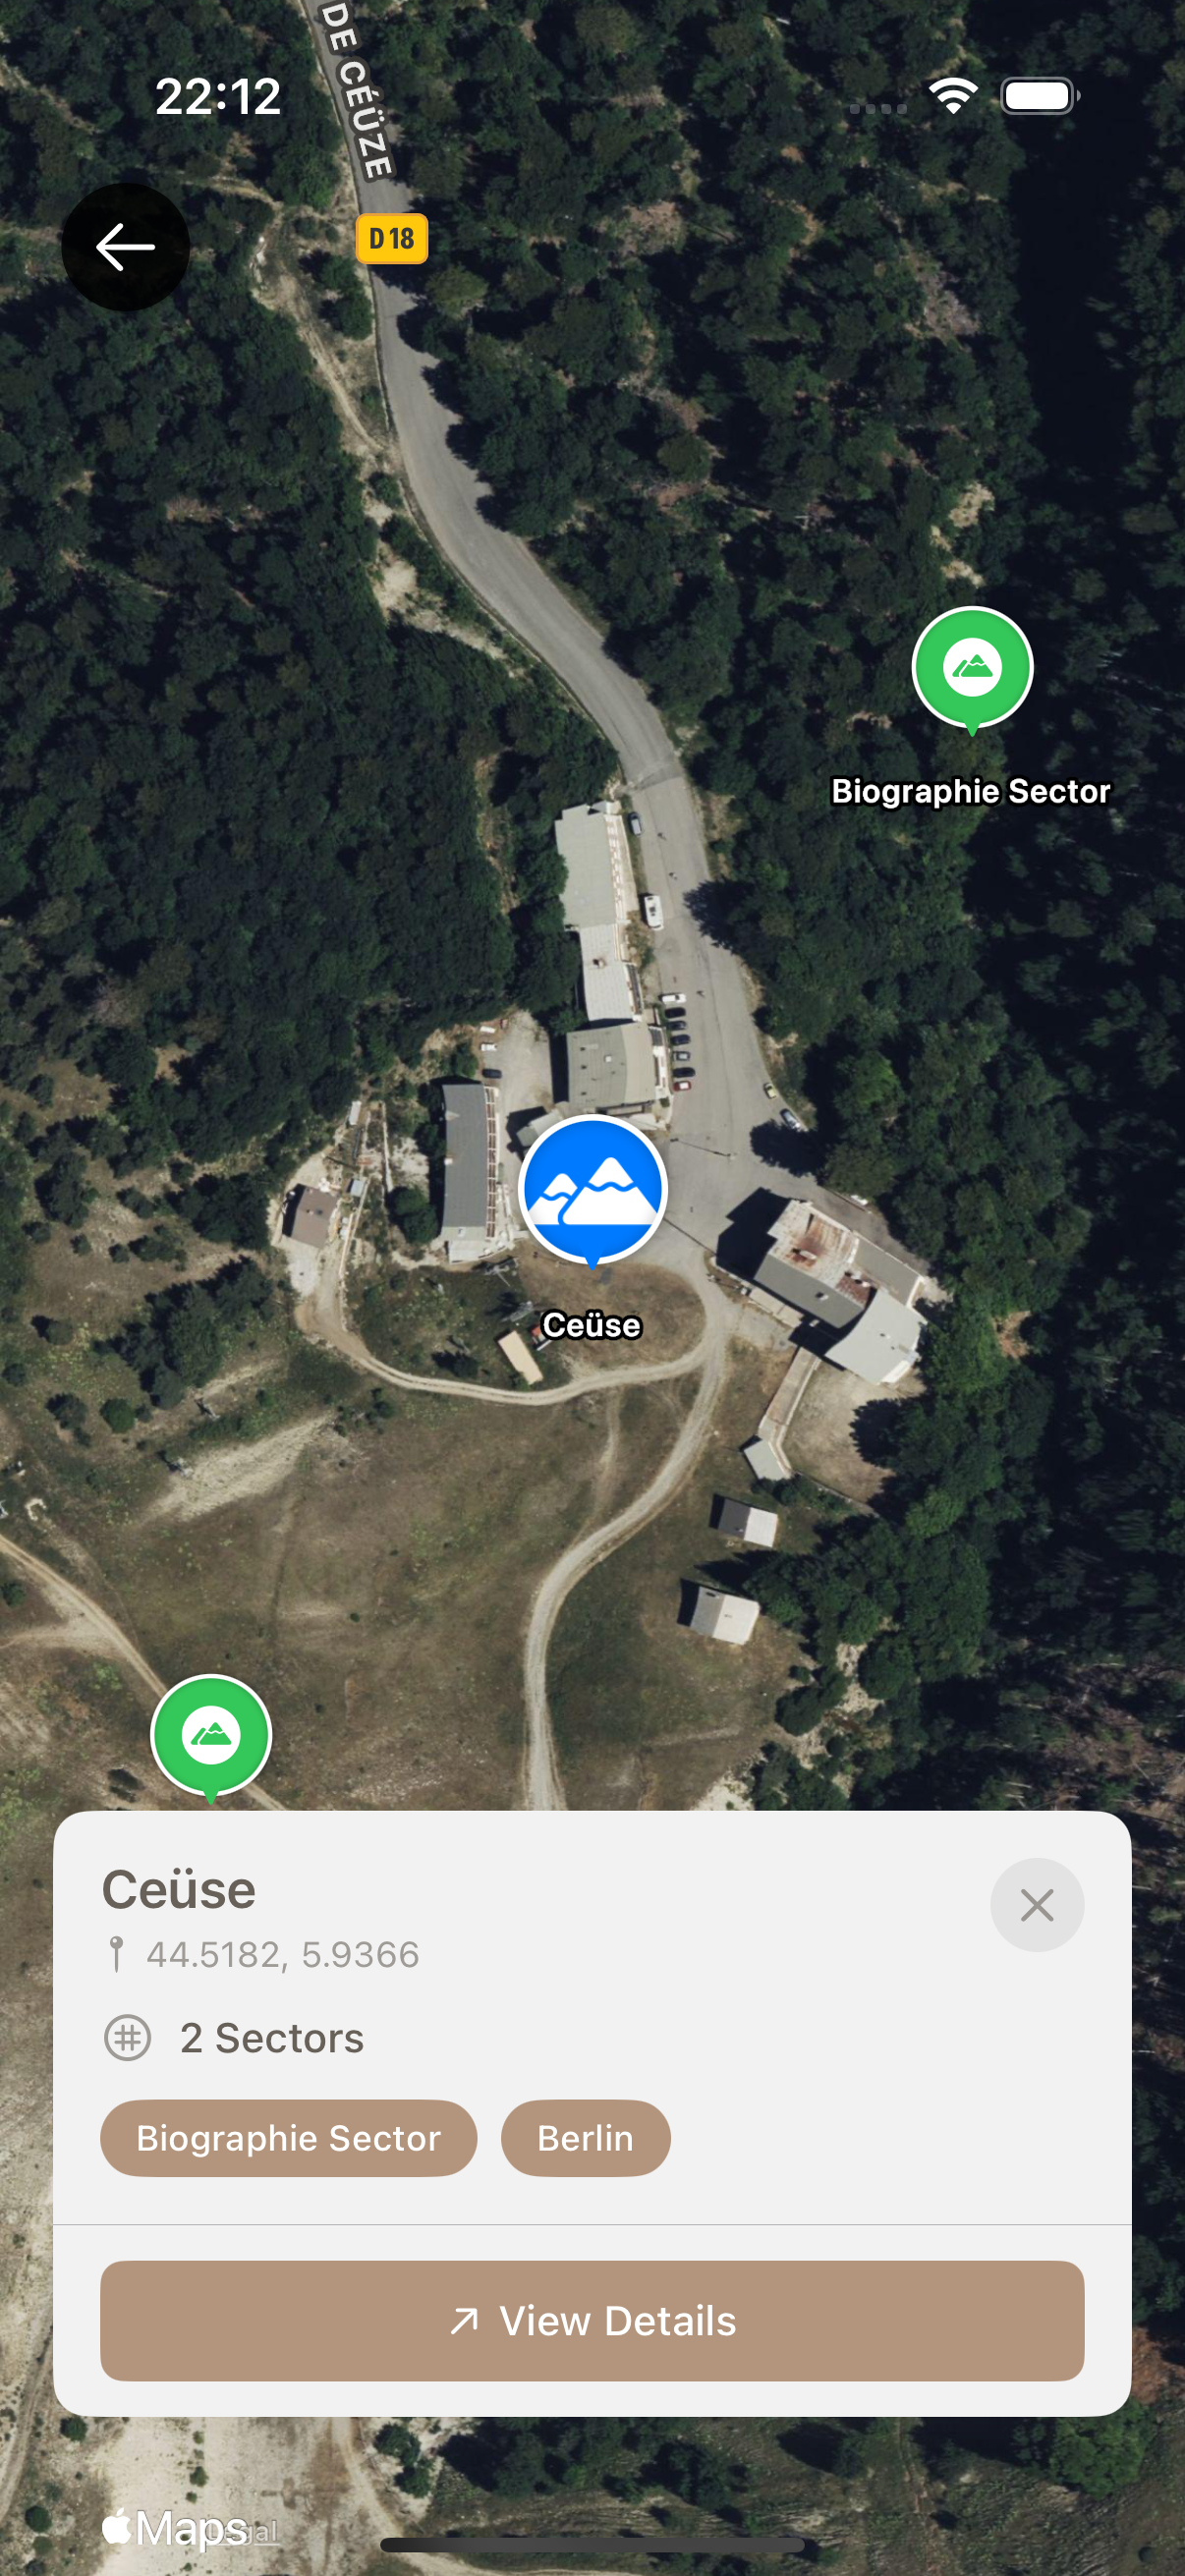
\includegraphics[width=0.3\textwidth]{images/implementacija/geo_karta_ceuse.png}
        \caption{Mobilna aplikacija}
        \label{fig:geografska_karta_ceuse_mob}
    \end{subfigure}
    \hfill
    \begin{subfigure}[b]{\textwidth}
        \centering
        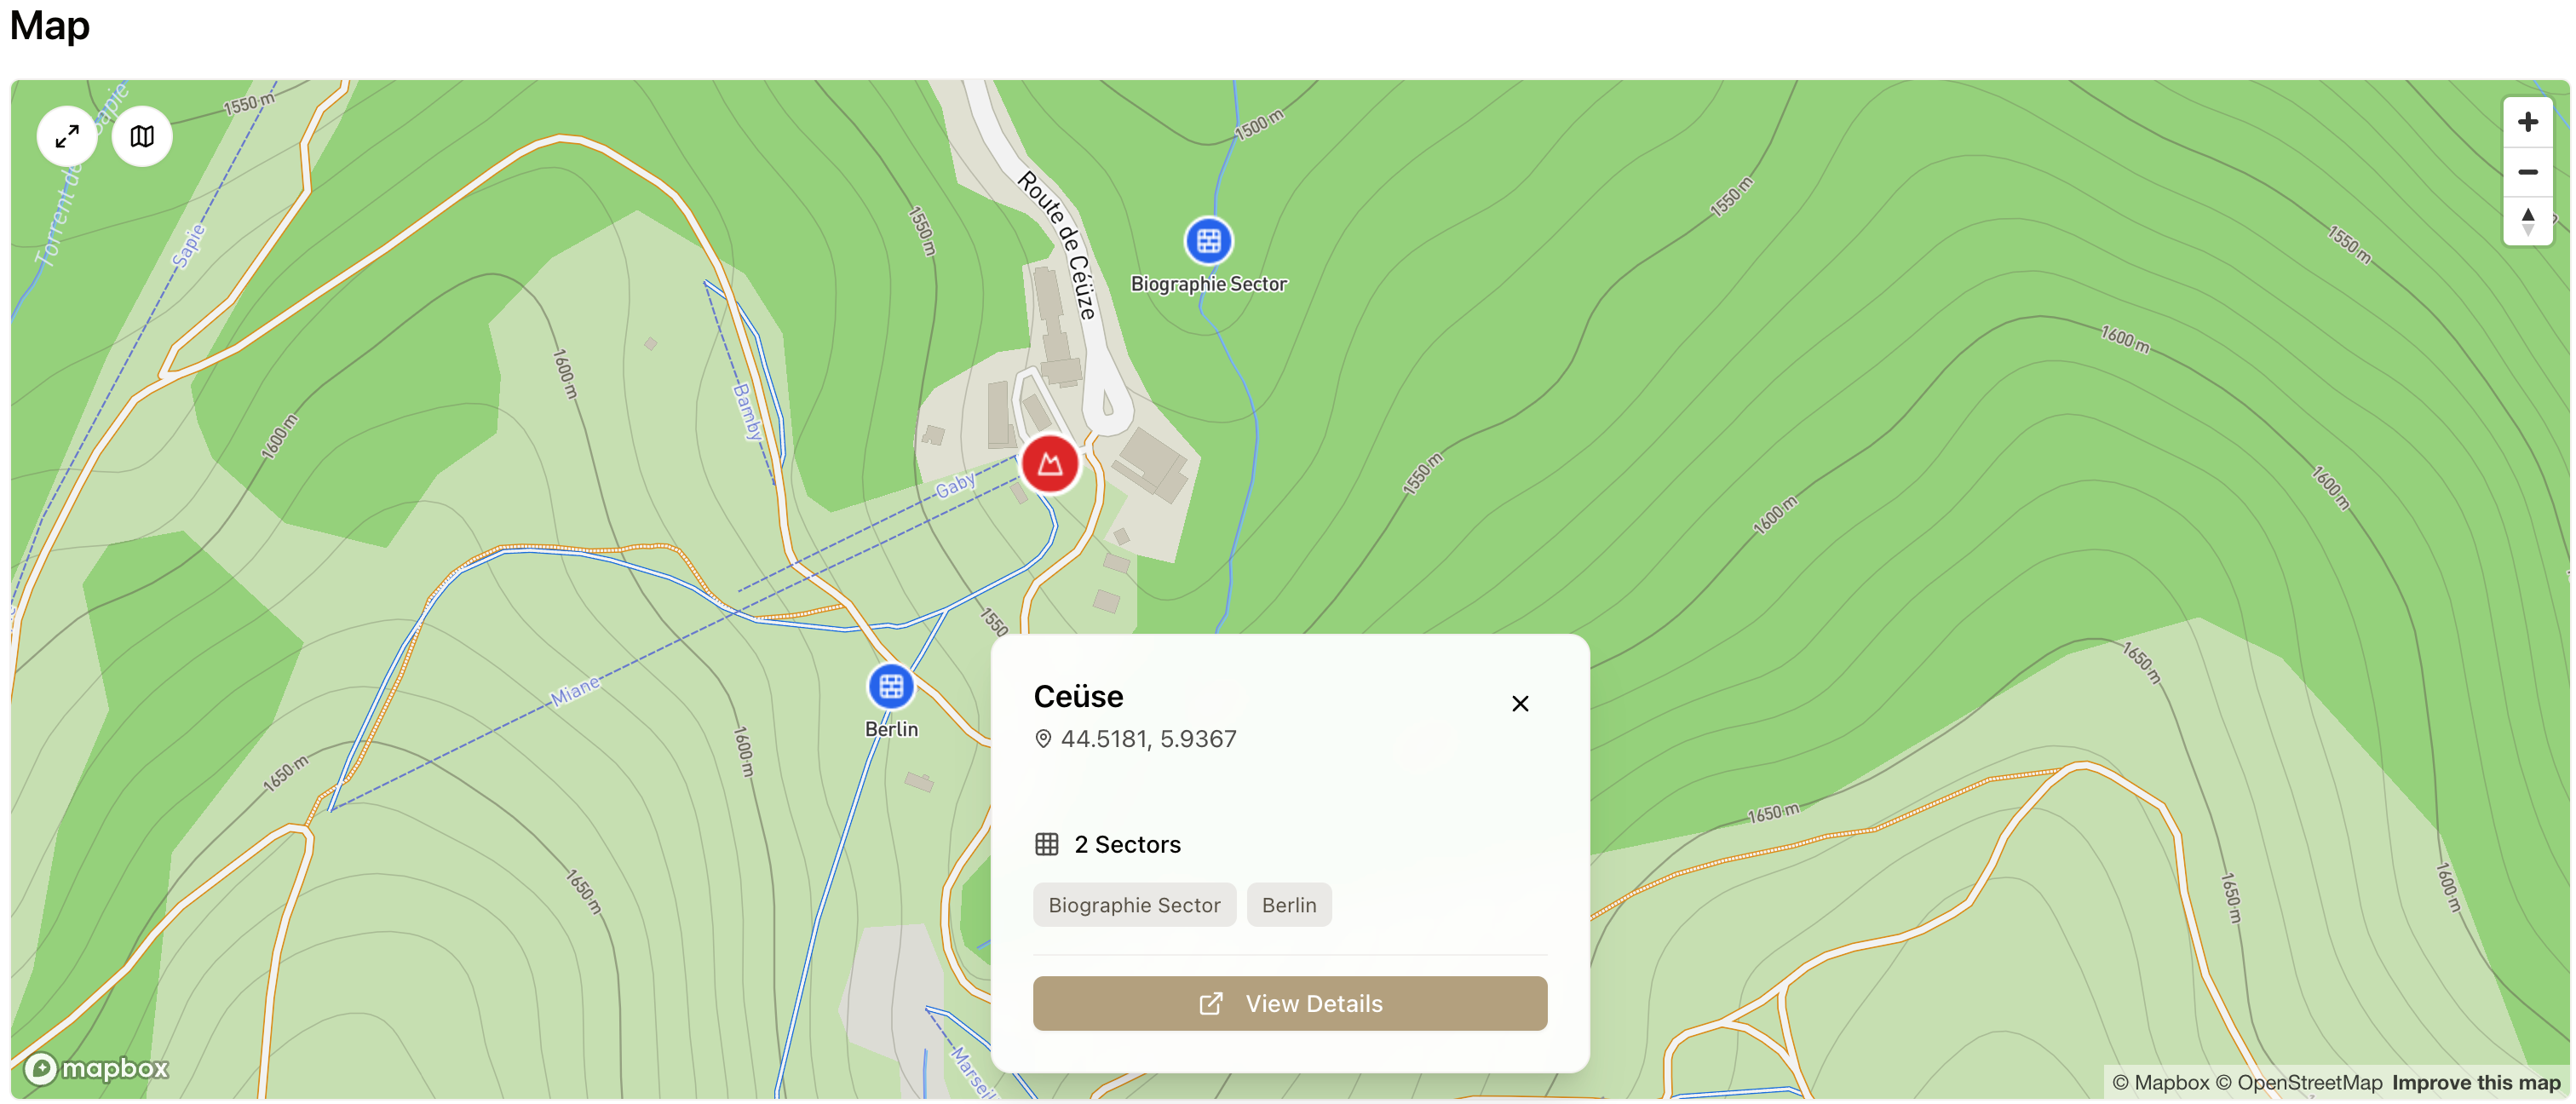
\includegraphics[width=0.9\textwidth]{images/implementacija/web/map_selected.png}
        \caption{Web aplikacija}
        \label{fig:geografska_karta_ceuse_web}
    \end{subfigure}
    \caption{Detaljan prikaz penjačke lokacije Ceuse}
    \label{fig:geografska_karta_ceuse_sidebyside}
\end{figure}

Odabirom oznake za pojedino penjalište, karta se automatski centrira i približava na tu lokaciju, prikazujući satelitski snimak područja. Na ovom detaljnom prikazu prikazana je oznaka za penjačku lokaciju, a i oznake za sve sektore. Ovakav prikaz je koristan za razumijevanje rasporeda sektora i planiranje kretanja na terenu. Na dnu prikaza nalazi se informativna kartica s osnovnim podacima o odabranoj lokaciji poput naziva, GPS koordinata i popisa dostupnih sektora. Korisniku se tada nude opcije za pregled detaljnih informacija o toj penjačkoj lokaciji ili sektorima. 
